\chapter{Mammography}
\label{ch:mammography}

% Chapter-opening illustrated modality infographic.
\begin{center}
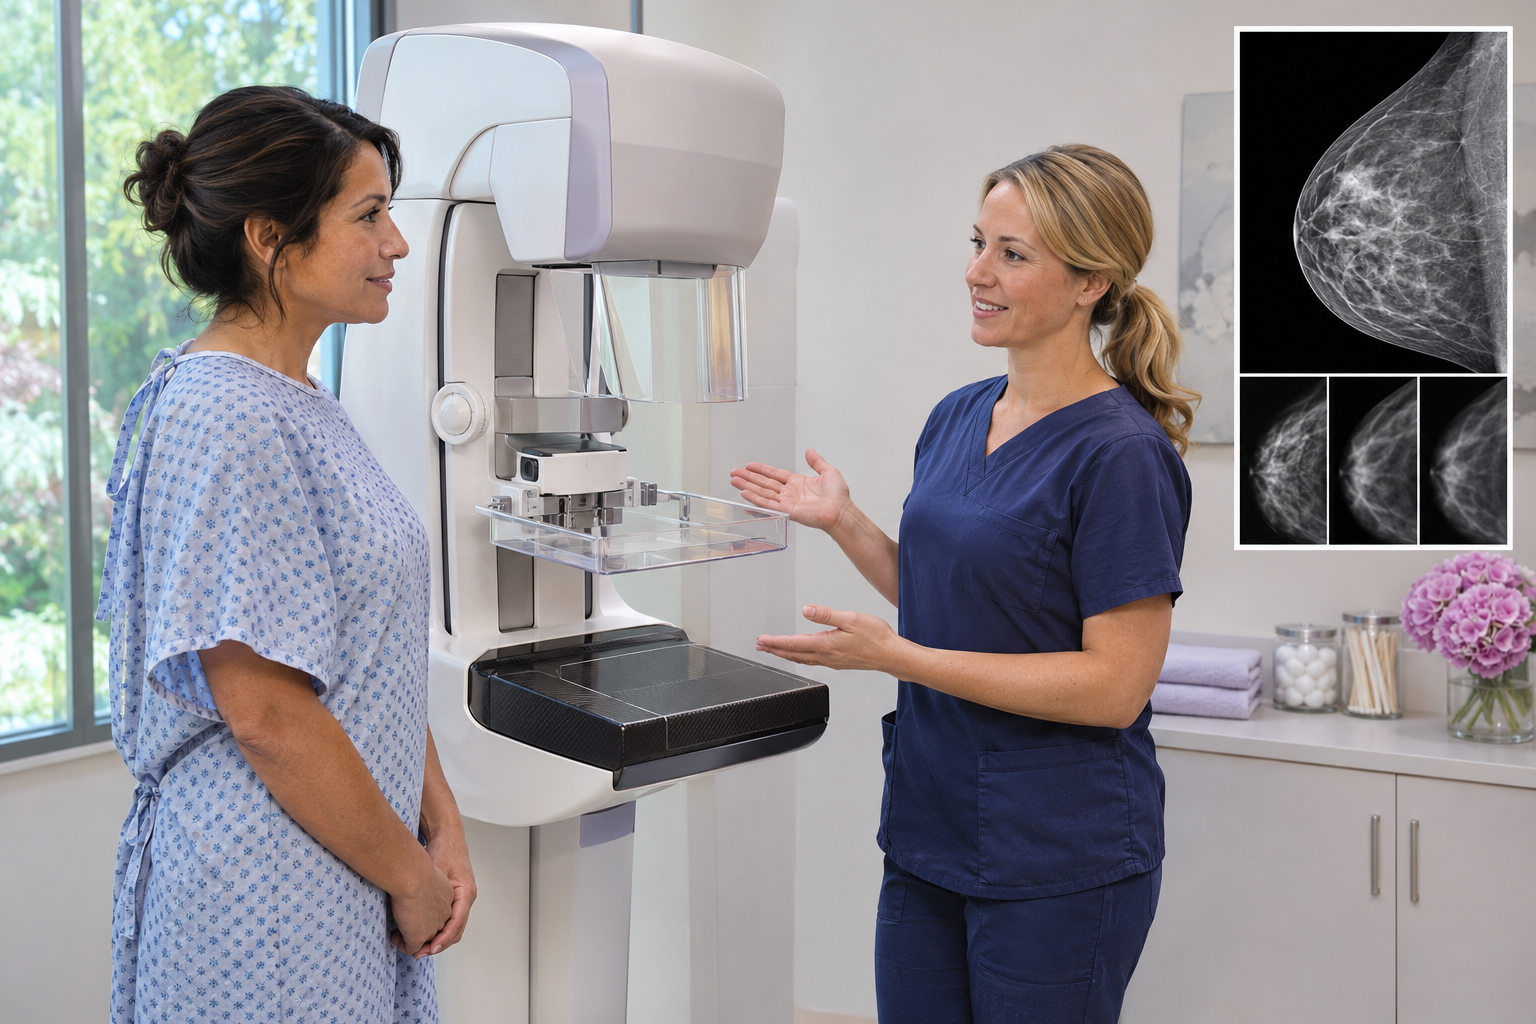
\includegraphics[width=\textwidth,keepaspectratio]{modalities/infographics/mammography_realistic.png}
\end{center}
\begin{center}\footnotesize Breast compression spreads tissue for low-dose X-ray projections; tomosynthesis reconstructs thin sections to reduce the effect of overlapping tissue. AI-generated illustration; mammogram inset is not a patient study.\end{center}

\section{Overview}
Digital mammography depicts masses, calcifications, and changes in the arrangement of breast tissue on low-dose X-ray projections. Digital breast tomosynthesis (DBT) reconstructs thin sections that can reveal a distortion hidden by overlapping tissue on a projection image.

\section{Where mammography is used}
The 80 entries include diseases, visible findings, and anatomical variants. Several share an appearance. For example, an irregular mass with radiating lines may represent invasive cancer, a radial scar, or a postoperative scar. Its location, prior images, and, when indicated, tissue sampling help establish the cause.

\subsection{Malignant breast diseases}
\begin{enumerate}[leftmargin=*,itemsep=0.45em,topsep=0.4em]
\item \textbf{Breast angiosarcoma.}\par\noindent\textbf{Symptoms:} A growing breast mass, skin discoloration, or a mass arising after breast irradiation may prompt diagnostic imaging.\par\noindent\textbf{Clinical Features:} A new mass or focal asymmetry; mammographic appearances are often nonspecific.\par\noindent\textbf{Role and sufficiency:} Mammography can localize the abnormality but cannot identify vascular histology; ultrasound/MRI and core biopsy are needed, and a negative mammogram does not exclude a clinically evident lesion.
\item \textbf{Carcinoma with medullary features.}\par\noindent\textbf{Symptoms:} A that can be felt rapidly growing mass or screening abnormality may prompt diagnostic views.\par\noindent\textbf{Clinical Features:} A round or oval high-density mass, sometimes circumscribed despite malignancy.\par\noindent\textbf{Role and sufficiency:} Imaging raises or lowers suspicion but cannot establish medullary shape; tissue diagnosis is required.
\item \textbf{Ductal carcinoma in situ (DCIS).}\par\noindent\textbf{Symptoms:} Screening commonly detects nonthat can be felt calcifications before symptoms develop.\par\noindent\textbf{Clinical Features:} Fine pleomorphic or fine linear/branching calcifications, particularly in a segmental or linear distribution; assess extent on magnification views.\par\noindent\textbf{Role and sufficiency:} Mammography is the principal detection method for calcified DCIS, but biopsy is required; noncalcified DCIS can be occult, and MRI may help assess extent in selected cases.
\item \textbf{Inflammatory breast cancer.}\par\noindent\textbf{Symptoms:} Rapid diffuse redness, edema, peau d'orange, or breast enlargement may prompt urgent diagnostic imaging.\par\noindent\textbf{Clinical Features:} Skin and trabecular thickening, increased density, asymmetry, and possible mass or abnormal nodes.\par\noindent\textbf{Role and sufficiency:} Findings overlap with mastitis and a discrete mass may be absent; clinical course and skin/core biopsy establish diagnosis, so a negative mammogram must not delay evaluation.
\item \textbf{Invasive carcinoma of no special type (invasive ductal carcinoma).}\par\noindent\textbf{Symptoms:} A screening recall, new lump, or focal symptom may lead to diagnostic mammography.\par\noindent\textbf{Clinical Features:} Irregular high-density mass, with thin lines radiating from its edge margins, architectural distortion, or suspicious calcifications; compare with prior studies.\par\noindent\textbf{Role and sufficiency:} Mammography detects and maps many lesions but cannot distinguish cancer from all scars or benign mimics; targeted ultrasound and image-guided biopsy establish diagnosis.
\item \textbf{Invasive lobular carcinoma.}\par\noindent\textbf{Symptoms:} A subtle that can be felt thickening, asymmetry, or screening change may prompt diagnostic mammography, often with DBT.\par\noindent\textbf{Clinical Features:} Architectural distortion, developing asymmetry, or subtle ill-defined density; bilateral comparison is useful.\par\noindent\textbf{Role and sufficiency:} This tumor may be mammographically occult or underestimated; targeted ultrasound and MRI are often used to define extent, while biopsy confirms it.
\item \textbf{Malignant phyllodes tumor.}\par\noindent\textbf{Symptoms:} A rapidly enlarging that can be felt mass may prompt diagnostic imaging.\par\noindent\textbf{Clinical Features:} A large oval or lobulated mass, sometimes with clefts or heterogeneous density.\par\noindent\textbf{Role and sufficiency:} Imaging cannot reliably distinguish benign, borderline, and malignant phyllodes tumors; core or excision pathology determines grade.
\item \textbf{Metaplastic breast carcinoma.}\par\noindent\textbf{Symptoms:} A rapidly enlarging that can be felt mass may prompt diagnostic mammography and ultrasound.\par\noindent\textbf{Clinical Features:} A dense irregular or occasionally circumscribed mass, with possible necrotic or cystic components on ultrasound.\par\noindent\textbf{Role and sufficiency:} Appearance is variable and may mimic benign disease; biopsy is necessary to identify metaplastic differentiation.
\item \textbf{Metastases to the breast.}\par\noindent\textbf{Symptoms:} A new breast lump in a patient with known extramammary cancer may prompt targeted imaging.\par\noindent\textbf{Clinical Features:} One or multiple round or oval masses, often without the spiculation or calcifications of a primary breast cancer.\par\noindent\textbf{Role and sufficiency:} Appearance cannot reliably determine origin; comparison with cancer history and tissue sampling are needed, with systemic staging guided by the primary disease.
\item \textbf{Mucinous carcinoma.}\par\noindent\textbf{Symptoms:} A that can be felt lump or screening-detected mass may prompt diagnostic views.\par\noindent\textbf{Clinical Features:} A lobulated, sometimes circumscribed mass; calcifications are less typical.\par\noindent\textbf{Role and sufficiency:} A deceptively circumscribed margin does not exclude cancer, and mammography cannot identify mucinous histology; biopsy is required.
\item \textbf{Paget disease of the breast.}\par\noindent\textbf{Symptoms:} Persistent unilateral nipple eczema, scaling, erosion, or discharge prompts evaluation for underlying carcinoma.\par\noindent\textbf{Clinical Features:} Nipple-areolar thickening or retraction, behind the nipple mass, and suspicious calcifications.\par\noindent\textbf{Role and sufficiency:} Mammography can identify associated disease but may be normal; persistent nipple changes require clinical assessment and skin biopsy, with ultrasound/MRI as indicated.
\item \textbf{Papillary carcinoma.}\par\noindent\textbf{Symptoms:} A that can be felt behind the nipple mass or bloody nipple discharge may prompt diagnostic mammography.\par\noindent\textbf{Clinical Features:} A circumscribed or irregular mass, asymmetry, or associated calcifications.\par\noindent\textbf{Role and sufficiency:} Imaging cannot reliably separate benign papilloma from papillary carcinoma or define subtype; targeted ultrasound and tissue sampling are required.
\item \textbf{Primary breast lymphoma.}\par\noindent\textbf{Symptoms:} A rapidly enlarging breast mass or unexplained breast asymmetry may prompt diagnostic imaging, especially with known lymphoma.\par\noindent\textbf{Clinical Features:} A dense, often noncalcified mass or diffuse asymmetry; nodal findings may coexist.\par\noindent\textbf{Role and sufficiency:} Mammography is nonspecific and cannot establish lymphoma or whether it is primary; biopsy with immunophenotyping and systemic staging are essential.
\item \textbf{Tubular carcinoma.}\par\noindent\textbf{Symptoms:} A small screening-detected distortion or mass may prompt diagnostic magnification views and DBT.\par\noindent\textbf{Clinical Features:} A small with thin lines radiating from its edge lesion, sometimes with architectural distortion.\par\noindent\textbf{Role and sufficiency:} It can resemble radial scar or other invasive cancer; biopsy is required for histology and imaging alone cannot determine subtype.
\end{enumerate}

\subsection{High-risk lesions and benign mimics}
\begin{enumerate}[leftmargin=*,itemsep=0.45em,topsep=0.4em]
\item \textbf{Atypical ductal hyperplasia (ADH).}\par\noindent\textbf{Symptoms:} Screening-detected calcifications or a mammographic target may prompt stereotactic biopsy.\par\noindent\textbf{Clinical Features:} Grouped calcifications, often amorphous or fine pleomorphic; ADH itself is a microscopic biopsy diagnosis.\par\noindent\textbf{Role and sufficiency:} Mammography identifies the target but cannot diagnose ADH or reliably separate it from DCIS; pathology and imaging--pathology concordance guide management.
\item \textbf{Atypical lobular hyperplasia (ALH).}\par\noindent\textbf{Symptoms:} Imaging is usually obtained for a separate screening or diagnostic finding, with ALH discovered on biopsy.\par\noindent\textbf{Clinical Features:} Assess whether the mammographic target is fully sampled and whether the imaging abnormality persists.\par\noindent\textbf{Role and sufficiency:} ALH has no specific mammographic appearance; imaging cannot diagnose it, and management depends on pathology, concordance, and risk context.
\item \textbf{Complex sclerosing lesion.}\par\noindent\textbf{Symptoms:} A screening distortion or suspicious asymmetry may prompt diagnostic views and biopsy.\par\noindent\textbf{Clinical Features:} Stellate architectural distortion with radiating lines, sometimes without a central mass.\par\noindent\textbf{Role and sufficiency:} It can mimic invasive carcinoma and imaging cannot distinguish them; core sampling and concordance are needed, with excision considered according to pathology and sampling adequacy.
\item \textbf{Flat epithelial atypia.}\par\noindent\textbf{Symptoms:} Grouped calcifications found at screening may be sampled stereotactically.\par\noindent\textbf{Clinical Features:} The shape and distribution of calcifications that define the biopsy target; the epithelial atypia is not visible on the image.\par\noindent\textbf{Role and sufficiency:} Mammography detects the target but cannot identify flat epithelial atypia; tissue results and concordance determine whether further sampling is warranted.
\item \textbf{Lobular carcinoma in situ (LCIS).}\par\noindent\textbf{Symptoms:} Imaging is performed for a screening abnormality or risk-based surveillance, with classic LCIS often an incidental biopsy finding.\par\noindent\textbf{Clinical Features:} Pleomorphic or florid LCIS may be associated with suspicious calcifications; classic LCIS often has no imaging correlate.\par\noindent\textbf{Role and sufficiency:} Mammography cannot diagnose LCIS; biopsy subtype, extent, and concordance determine management.
\item \textbf{Papilloma with atypia.}\par\noindent\textbf{Symptoms:} A mass, asymmetry, calcifications, or pathologic nipple discharge may prompt diagnostic imaging and biopsy.\par\noindent\textbf{Clinical Features:} A behind the nipple mass or duct-related abnormality; calcifications may also be present.\par\noindent\textbf{Role and sufficiency:} Mammography cannot detect the atypia or reliably separate papilloma from carcinoma; ultrasound and tissue sampling are needed.
\item \textbf{Radial scar.}\par\noindent\textbf{Symptoms:} A screening-detected distortion or with thin lines radiating from its edge lesion may prompt additional views, DBT, and biopsy.\par\noindent\textbf{Clinical Features:} Radiating lines converging toward a central lucency or density, often without a discrete mass.\par\noindent\textbf{Role and sufficiency:} The appearance overlaps with carcinoma; biopsy establishes the lesion and associated atypia, with management based on radiology-pathology concordance.
\end{enumerate}

\subsection{Benign breast tumors and masses}
\begin{enumerate}[leftmargin=*,itemsep=0.45em,topsep=0.4em]
\item \textbf{Benign adenomyoepithelioma.}\par\noindent\textbf{Symptoms:} A that can be felt lump or screening-detected mass may prompt diagnostic views.\par\noindent\textbf{Clinical Features:} An oval, lobulated, or irregular mass, with margins and interval growth carefully assessed.\par\noindent\textbf{Role and sufficiency:} Appearance overlaps with malignant and other benign tumors; biopsy is needed to distinguish benign, atypical, and malignant forms.
\item \textbf{Benign phyllodes tumor.}\par\noindent\textbf{Symptoms:} A rapidly enlarging that can be felt mass may prompt diagnostic imaging.\par\noindent\textbf{Clinical Features:} A circumscribed, often lobulated mass that may be large and heterogeneous.\par\noindent\textbf{Role and sufficiency:} Mammography cannot reliably separate phyllodes tumor from fibroadenoma or determine grade; tissue diagnosis is needed.
\item \textbf{Breast hamartoma.}\par\noindent\textbf{Symptoms:} A that can be felt lump or screening asymmetry may prompt mammography.\par\noindent\textbf{Clinical Features:} A circumscribed mass containing mixed fat and fibroglandular tissue, sometimes with a thin pseudocapsule.\par\noindent\textbf{Role and sufficiency:} A classic appearance can be diagnostic, but atypical or changing lesions require targeted ultrasound and sometimes biopsy.
\item \textbf{Breast hemangioma.}\par\noindent\textbf{Symptoms:} A that can be felt or incidental mass may prompt diagnostic imaging.\par\noindent\textbf{Clinical Features:} A circumscribed mass, sometimes with calcifications, without a reliably specific pattern.\par\noindent\textbf{Role and sufficiency:} Mammography cannot establish vascular histology; ultrasound/Doppler and, when needed, biopsy characterize an indeterminate lesion.
\item \textbf{Breast lipoma.}\par\noindent\textbf{Symptoms:} A that can be felt soft mass or incidental lesion may be assessed on mammography.\par\noindent\textbf{Clinical Features:} A circumscribed radiolucent mass with a thin capsule and no suspicious solid component.\par\noindent\textbf{Role and sufficiency:} A classic fat-containing appearance is usually sufficient; atypical density or discordant examination warrants further imaging.
\item \textbf{Breast myofibroblastoma.}\par\noindent\textbf{Symptoms:} A slowly growing that can be felt mass may prompt diagnostic mammography.\par\noindent\textbf{Clinical Features:} A circumscribed or mildly lobulated soft-tissue density, sometimes with coarse calcification.\par\noindent\textbf{Role and sufficiency:} The appearance is nonspecific and cannot identify this stromal tumor; core biopsy establishes the diagnosis.
\item \textbf{Fibroadenoma.}\par\noindent\textbf{Symptoms:} A that can be felt lump or screening-detected mass may lead to diagnostic assessment, especially in older patients.\par\noindent\textbf{Clinical Features:} An oval or gently lobulated circumscribed mass; involution may produce coarse popcorn-like calcification.\par\noindent\textbf{Role and sufficiency:} A stable classic lesion may be characterized with ultrasound and prior comparison, but mammography alone cannot prove fibroadenoma when features are new or suspicious.
\item \textbf{Granular cell tumor.}\par\noindent\textbf{Symptoms:} A firm that can be felt lump or imaging abnormality may prompt diagnostic views.\par\noindent\textbf{Clinical Features:} An irregular mass or architectural distortion, sometimes with thin lines radiating from its edge and indistinguishable from cancer.\par\noindent\textbf{Role and sufficiency:} Imaging cannot distinguish this benign tumor from carcinoma; biopsy is required.
\item \textbf{Intraductal papilloma.}\par\noindent\textbf{Symptoms:} Bloody nipple discharge or a behind the nipple lump may prompt diagnostic mammography and targeted ultrasound.\par\noindent\textbf{Clinical Features:} A behind the nipple mass, focal asymmetry, or duct-associated calcifications; small papillomas may be occult.\par\noindent\textbf{Role and sufficiency:} Mammography may miss the lesion and cannot determine atypia; ultrasound, duct evaluation, and tissue sampling are considered based on symptoms and findings.
\item \textbf{Involuting fibroadenoma.}\par\noindent\textbf{Symptoms:} Screening or follow-up may show progressive calcification within a known mass.\par\noindent\textbf{Clinical Features:} Coarse, dense, popcorn-like calcifications developing within a circumscribed lesion.\par\noindent\textbf{Role and sufficiency:} A classic evolution is benign and often needs no biopsy; suspicious shape or discordant change requires diagnostic assessment.
\item \textbf{Pseudoangiomatous stromal hyperplasia (PASH).}\par\noindent\textbf{Symptoms:} A that can be felt enlarging mass or screening asymmetry may prompt diagnostic imaging.\par\noindent\textbf{Clinical Features:} A circumscribed mass or focal asymmetry; microscopic PASH may have no visible correlate.\par\noindent\textbf{Role and sufficiency:} Imaging is nonspecific and cannot establish PASH; core biopsy and concordance determine whether the result explains the finding.
\item \textbf{Tubular adenoma.}\par\noindent\textbf{Symptoms:} A that can be felt lump or screening mass may prompt diagnostic views.\par\noindent\textbf{Clinical Features:} A circumscribed, often oval mass; calcifications may occur.\par\noindent\textbf{Role and sufficiency:} Its appearance overlaps with fibroadenoma and other lesions; biopsy is needed when imaging is not characteristically benign.
\end{enumerate}

\subsection{Cystic and fibrocystic breast conditions}
\begin{enumerate}[leftmargin=*,itemsep=0.45em,topsep=0.4em]
\item \textbf{Apocrine metaplasia.}\par\noindent\textbf{Symptoms:} Imaging may be obtained for a cyst, calcifications, or that can be felt finding, with apocrine change identified incidentally on pathology.\par\noindent\textbf{Clinical Features:} Describe the associated cystic lesion or calcification pattern; apocrine metaplasia has no specific mammographic sign.\par\noindent\textbf{Role and sufficiency:} Mammography cannot diagnose the microscopic change; pathology and concordance determine whether it explains the target.
\item \textbf{Breast adenosis.}\par\noindent\textbf{Symptoms:} A screening asymmetry, mass, or calcification may prompt diagnostic assessment.\par\noindent\textbf{Clinical Features:} Focal asymmetry, small masses, or calcifications, which vary with the subtype.\par\noindent\textbf{Role and sufficiency:} These findings are nonspecific and can mimic malignancy; targeted ultrasound and biopsy are used when suspicious, while pathology identifies adenosis.
\item \textbf{Complicated breast cyst.}\par\noindent\textbf{Symptoms:} A that can be felt lump or circumscribed mammographic mass may prompt targeted ultrasound.\par\noindent\textbf{Clinical Features:} On mammography, a round or oval circumscribed mass; ultrasound assesses mobile debris, wall features, and whether a solid component exists.\par\noindent\textbf{Role and sufficiency:} Mammography cannot reliably distinguish a complicated cyst from a solid mass; ultrasound is the key characterization test and suspicious solid components may require biopsy.
\item \textbf{Fibrocystic breast changes.}\par\noindent\textbf{Symptoms:} Cyclic nodularity, focal pain, or screening abnormalities may prompt diagnostic imaging.\par\noindent\textbf{Clinical Features:} Multiple circumscribed masses, focal asymmetries, or calcifications; evaluate each dominant or new finding rather than attributing all changes to a general pattern.\par\noindent\textbf{Role and sufficiency:} Mammography describes visible findings but does not establish a single fibrocystic diagnosis or dismiss a suspicious focal lesion; ultrasound may clarify cystic masses.
\item \textbf{Galactocele.}\par\noindent\textbf{Symptoms:} A persistent lump during lactation or after weaning may prompt imaging.\par\noindent\textbf{Clinical Features:} A circumscribed mass with a fat-fluid level when visible, correlating with lactation history.\par\noindent\textbf{Role and sufficiency:} This appearance can be characteristic, but ultrasound is often preferred during lactation and evaluates internal contents; atypical or persistent lesions need further assessment.
\item \textbf{Oil cyst.}\par\noindent\textbf{Symptoms:} A that can be felt lump after surgery, trauma, or fat grafting may prompt diagnostic views.\par\noindent\textbf{Clinical Features:} A fat-density round mass, sometimes with a thin rim of calcification.\par\noindent\textbf{Role and sufficiency:} A classic oil cyst is a benign imaging diagnosis; irregular margins or an unexplained that can be felt abnormality require ultrasound and possible biopsy.
\item \textbf{Sclerosing adenosis.}\par\noindent\textbf{Symptoms:} Screening calcifications, a mass, or distortion may lead to diagnostic imaging and biopsy.\par\noindent\textbf{Clinical Features:} Grouped calcifications, focal asymmetry, or architectural distortion.\par\noindent\textbf{Role and sufficiency:} It can closely mimic carcinoma; imaging cannot confirm sclerosing adenosis, and tissue diagnosis with concordance is needed for suspicious findings.
\item \textbf{Simple breast cyst.}\par\noindent\textbf{Symptoms:} A that can be felt lump or screening-detected circumscribed mass may prompt diagnostic assessment.\par\noindent\textbf{Clinical Features:} A round or oval circumscribed mass; targeted ultrasound demonstrates a thin wall and anechoic fluid with posterior enhancement.\par\noindent\textbf{Role and sufficiency:} Mammography alone cannot prove simple fluid; a classic ultrasound appearance is generally sufficient, while complex features prompt further evaluation.
\end{enumerate}

Debris can move within a complicated cyst. A discrete solid component on ultrasound raises a different diagnostic question and is described as part of a complex cystic and solid mass.

\subsection{Inflammatory and infectious conditions}
\begin{enumerate}[leftmargin=*,itemsep=0.45em,topsep=0.4em]
\item \textbf{Breast abscess.}\par\noindent\textbf{Symptoms:} A painful red swelling or persistent focal lump may prompt imaging, particularly if the patient is outside the usual lactational setting or does not improve.\par\noindent\textbf{Clinical Features:} Focal asymmetry, skin thickening, and surrounding edema; targeted ultrasound identifies a drainable complex collection.\par\noindent\textbf{Role and sufficiency:} Mammography cannot reliably separate abscess from inflammatory cancer; ultrasound and clinical assessment guide drainage, with biopsy or reassessment for persistent abnormalities.
\item \textbf{Breast edema.}\par\noindent\textbf{Symptoms:} Diffuse swelling, peau d'orange, or skin thickening may prompt diagnostic views to assess extent and associated lesion.\par\noindent\textbf{Clinical Features:} Skin and trabecular thickening, increased density, and asymmetry compared with prior images.\par\noindent\textbf{Role and sufficiency:} These signs are nonspecific and occur with infection, treatment, heart failure, or lymphatic obstruction; clinical context and targeted imaging determine cause.
\item \textbf{Breast tuberculosis.}\par\noindent\textbf{Symptoms:} A chronic lump, sinus, or skin change in an appropriate epidemiologic context may prompt imaging.\par\noindent\textbf{Clinical Features:} Irregular mass, asymmetry, skin thickening, or abnormal nodes; none is specific for tuberculosis.\par\noindent\textbf{Role and sufficiency:} Mammography cannot identify the organism or reliably distinguish cancer; tissue sampling for histology and microbiology is required.
\item \textbf{Diabetic mastopathy.}\par\noindent\textbf{Symptoms:} A firm that can be felt mass in a person with long-standing diabetes may prompt diagnostic imaging.\par\noindent\textbf{Clinical Features:} Dense tissue, focal asymmetry, or an irregular mass; the lesion may also be occult.\par\noindent\textbf{Role and sufficiency:} Imaging can mimic carcinoma and diabetes does not explain away suspicious features; ultrasound-guided core biopsy is often needed for a new indeterminate mass.
\item \textbf{Granulomatous mastitis.}\par\noindent\textbf{Symptoms:} Painful mass, erythema, or recurrent inflammatory change may prompt imaging when symptoms persist or are atypical.\par\noindent\textbf{Clinical Features:} Asymmetry, irregular masses, skin thickening, or sinus-related changes.\par\noindent\textbf{Role and sufficiency:} Findings can resemble invasive cancer or infection; biopsy and microbiological assessment help establish cause, and follow-up confirms resolution.
\item \textbf{Mammary duct ectasia.}\par\noindent\textbf{Symptoms:} Nipple discharge, behind the nipple discomfort, or a subareolar lump may prompt diagnostic imaging.\par\noindent\textbf{Clinical Features:} Dilated behind the nipple ducts and smooth large rod-like secretory calcifications.\par\noindent\textbf{Role and sufficiency:} Mammography can show duct-related calcifications, but ultrasound better evaluates duct contents; suspicious discharge or intraductal mass needs targeted workup.
\item \textbf{Mastitis.}\par\noindent\textbf{Symptoms:} Persistent focal inflammation, a mass, or failure to improve with treatment may prompt imaging to look for an abscess or alternate diagnosis.\par\noindent\textbf{Clinical Features:} Skin/trabecular thickening, increased density, and focal asymmetry.\par\noindent\textbf{Role and sufficiency:} These are nonspecific and do not distinguish infection from inflammatory cancer; ultrasound evaluates a collection, and persistent change requires reassessment and possible biopsy.
\item \textbf{Periductal mastitis.}\par\noindent\textbf{Symptoms:} Recurrent subareolar pain, discharge, or inflammation may prompt diagnostic assessment.\par\noindent\textbf{Clinical Features:} Retroareolar asymmetry, duct widening, or associated mass; compare with the symptomatic side and prior studies.\par\noindent\textbf{Role and sufficiency:} Mammography is not specific for periductal inflammation; targeted ultrasound and clinical follow-up assess abscess or an alternative lesion.
\end{enumerate}

\subsection{Traumatic and postoperative conditions}
\begin{enumerate}[leftmargin=*,itemsep=0.45em,topsep=0.4em]
\item \textbf{Breast hematoma.}\par\noindent\textbf{Symptoms:} A new lump or bruising after trauma, biopsy, or surgery may prompt diagnostic imaging.\par\noindent\textbf{Clinical Features:} A focal mass or asymmetry and its evolution on prior or follow-up studies; ultrasound can show evolving internal echoes.\par\noindent\textbf{Role and sufficiency:} A resolving appearance supports hematoma, but a persistent or enlarging mass needs further evaluation because bleeding can obscure an underlying lesion.
\item \textbf{Extracapsular silicone implant rupture.}\par\noindent\textbf{Symptoms:} Pain, change in implant contour, or concern for implant complication may prompt imaging.\par\noindent\textbf{Clinical Features:} Silicone outside the implant capsule, sometimes as dense deposits in breast tissue or nodes.\par\noindent\textbf{Role and sufficiency:} Mammography may show extracapsular silicone but is insensitive for intracapsular rupture; implant-protocol MRI or ultrasound is preferred to assess integrity.
\item \textbf{Fat necrosis.}\par\noindent\textbf{Symptoms:} A that can be felt lump after surgery, trauma, or radiation may prompt diagnostic views.\par\noindent\textbf{Clinical Features:} Oil cyst, fat-containing mass, or thin rim calcification; irregular spiculation or evolving distortion is less reassuring.\par\noindent\textbf{Role and sufficiency:} Classic fat-containing findings can establish a benign explanation, but suspicious or discordant lesions require biopsy because fat necrosis can mimic cancer.
\item \textbf{Postoperative scarring.}\par\noindent\textbf{Symptoms:} Surveillance or a new that can be felt finding after breast surgery may prompt comparison with baseline postoperative studies.\par\noindent\textbf{Clinical Features:} Distortion at the operative bed and whether it remains stable or becomes more conspicuous.\par\noindent\textbf{Role and sufficiency:} Stable scar is often characterized by comparison; new or progressive distortion warrants diagnostic views, ultrasound, and possible biopsy.
\item \textbf{Postoperative seroma.}\par\noindent\textbf{Symptoms:} A that can be felt swelling after surgery may prompt assessment of the operative site.\par\noindent\textbf{Clinical Features:} A circumscribed mass at the surgical bed; ultrasound determines whether it is fluid-filled.\par\noindent\textbf{Role and sufficiency:} Mammography cannot confirm fluid contents; a typical ultrasound appearance and expected clinical course may suffice, while complex or persistent findings need further workup.
\item \textbf{Radiation-induced fibrosis.}\par\noindent\textbf{Symptoms:} Follow-up after breast irradiation evaluates expected treatment change and detects recurrence.\par\noindent\textbf{Clinical Features:} Late volume loss, retraction, and stable distortion; early skin/trabecular thickening can reflect edema.\par\noindent\textbf{Role and sufficiency:} Stability over serial examinations supports fibrosis, but new or progressive change requires targeted evaluation and sometimes biopsy.
\item \textbf{Silicone granuloma.}\par\noindent\textbf{Symptoms:} A that can be felt nodule or abnormal node in a patient with silicone implants may prompt diagnostic imaging.\par\noindent\textbf{Clinical Features:} Dense silicone deposits or nodules, including within regional lymph nodes.\par\noindent\textbf{Role and sufficiency:} Mammography can locate deposits but cannot confirm the granulomatous reaction or exclude malignancy; ultrasound/MRI and biopsy are used for indeterminate lesions.
\end{enumerate}

\subsection{Breast calcification patterns}
Describe both the shape of individual deposits and the distribution of the group. For example, fine pleomorphic deposits in a segmental distribution raise concern for a ductal process.

\begin{enumerate}[leftmargin=*,itemsep=0.45em,topsep=0.4em]
\item \textbf{Amorphous calcifications.}\par\noindent\textbf{Symptoms:} Screening detects calcifications that require diagnostic magnification views to characterize.\par\noindent\textbf{Clinical Features:} Tiny hazy particles whose shape is indistinct; document whether grouped, regional, linear, or segmental.\par\noindent\textbf{Role and sufficiency:} Distribution and comparison guide BI-RADS assessment, but suspicious grouped patterns generally require stereotactic biopsy; shape alone does not identify histology.
\item \textbf{Coarse calcifications.}\par\noindent\textbf{Symptoms:} A screening calcification cluster may prompt magnification views to determine whether deposits are characteristically benign.\par\noindent\textbf{Clinical Features:} Large, dense, often confluent deposits, including popcorn-like calcification in an involuting fibroadenoma or dystrophic calcification after injury.\par\noindent\textbf{Role and sufficiency:} A classic benign pattern is usually sufficient for benign classification; atypical shape or distribution may require additional assessment.
\item \textbf{Coarse heterogeneous calcifications.}\par\noindent\textbf{Symptoms:} Newly detected calcifications are characterized with magnification views and comparison.\par\noindent\textbf{Clinical Features:} Irregular, conspicuous particles with variable shape, typically smaller and less uniformly benign than coarse dystrophic deposits; assess distribution.\par\noindent\textbf{Role and sufficiency:} Suspicion depends on the group and context; mammography determines whether biopsy is warranted but cannot determine pathology.
\item \textbf{Fine linear or fine linear-branching calcifications.}\par\noindent\textbf{Symptoms:} Screening or diagnostic imaging detects a potentially ductal calcification pattern requiring workup.\par\noindent\textbf{Clinical Features:} Thin, irregular, discontinuous or branching deposits; map their linear or segmental distribution and extent.\par\noindent\textbf{Role and sufficiency:} This shape is suspicious and commonly prompts image-guided biopsy; mammography cannot establish DCIS or invasive disease.
\item \textbf{Fine pleomorphic calcifications.}\par\noindent\textbf{Symptoms:} Screening-detected calcifications are magnified to assess shape and distribution.\par\noindent\textbf{Clinical Features:} Small irregular particles varying in shape and size, with grouped, linear, or segmental arrangement recorded.\par\noindent\textbf{Role and sufficiency:} A suspicious pattern often requires stereotactic biopsy; image appearance estimates risk but does not provide tissue diagnosis.
\item \textbf{Large rod-like calcifications.}\par\noindent\textbf{Symptoms:} Nipple discharge or incidental ductal calcifications may prompt diagnostic review.\par\noindent\textbf{Clinical Features:} Smooth, elongated calcifications following a duct, often with a central lucency and behind the nipple predominance.\par\noindent\textbf{Role and sufficiency:} A classic bilateral secretory pattern is benign; unilateral, irregular, or associated mass findings require further evaluation.
\item \textbf{Layering calcifications (milk of calcium).}\par\noindent\textbf{Symptoms:} Indeterminate round calcifications may prompt magnification views, including a true lateral projection.\par\noindent\textbf{Clinical Features:} Dependent sediment in microcysts forming a crescent or teacup shape on the lateral view.\par\noindent\textbf{Role and sufficiency:} Demonstrated layering is a characteristic benign feature and can avoid biopsy; if layering is absent or shape remains suspicious, further assessment is needed.
\item \textbf{Rim calcifications.}\par\noindent\textbf{Symptoms:} A mass with peripheral calcification may be evaluated after trauma, surgery, or on screening.\par\noindent\textbf{Clinical Features:} Thin, smooth eggshell-like calcium outlining an oil cyst or other fat-containing lesion.\par\noindent\textbf{Role and sufficiency:} A classic rim pattern is benign; thick, irregular, or incomplete calcification around a suspicious mass should not be assumed benign.
\item \textbf{Skin calcifications.}\par\noindent\textbf{Symptoms:} Superficial calcifications may be recalled when their location is uncertain on standard views.\par\noindent\textbf{Clinical Features:} Deposits with central lucency; a tangential skin marker/view confirms superficial location.\par\noindent\textbf{Role and sufficiency:} Once confirmed as dermal, they are benign; without localization, they can be confused with intraparenchymal calcifications.
\item \textbf{Suture calcifications.}\par\noindent\textbf{Symptoms:} Calcifications near a surgical bed may prompt comparison with operative history and prior images.\par\noindent\textbf{Clinical Features:} Linear or knot-shaped deposits along a suture track, typically within a stable scar.\par\noindent\textbf{Role and sufficiency:} A typical postoperative pattern can be recognized on mammography; new suspicious calcifications outside the expected operative site need separate assessment.
\item \textbf{Vascular calcifications.}\par\noindent\textbf{Symptoms:} These are usually incidental findings on screening or diagnostic mammography.\par\noindent\textbf{Clinical Features:} Parallel, rail-like calcification along arterial walls rather than clustered ductal deposits.\par\noindent\textbf{Role and sufficiency:} Mammography readily identifies the vascular pattern but does not diagnose coronary artery disease; cardiovascular risk assessment is a separate clinical decision.
\end{enumerate}

\subsection{Structural findings and anatomical variants}
BI-RADS v2025 describes an asymmetry by its appearance on the current examination. Report separately whether it is new, larger, or more conspicuous on comparison with prior mammograms. An interval increase can warrant further assessment.
\begin{enumerate}[leftmargin=*,itemsep=0.45em,topsep=0.4em]
\item \textbf{Accessory breast tissue.}\par\noindent\textbf{Symptoms:} An axillary lump or focal swelling may prompt imaging to determine whether it is breast tissue or another lesion.\par\noindent\textbf{Clinical Features:} Fibroglandular tissue separate from the main breast, often in the axilla; the normal axillary tail remains continuous with breast tissue.\par\noindent\textbf{Role and sufficiency:} A characteristic appearance may establish ectopic tissue, but a discrete mass within it requires standard diagnostic evaluation.
\item \textbf{Architectural distortion.}\par\noindent\textbf{Symptoms:} Screening recall or a that can be felt thickening may prompt spot compression and DBT.\par\noindent\textbf{Clinical Features:} Converging lines or focal retraction without a definite mass, persistence across projections, and interval development.\par\noindent\textbf{Role and sufficiency:} DBT improves conspicuity but distortion is not a diagnosis; targeted ultrasound and biopsy are often needed to distinguish cancer from scar or radial scar.
\item \textbf{Asymmetry on one projection.}\par\noindent\textbf{Symptoms:} A density seen on only one screening view triggers recall to determine whether it represents overlap or a true lesion.\par\noindent\textbf{Clinical Features:} Whether the density persists on a second projection, spot compression, or DBT and whether it has a mass-like margin.\par\noindent\textbf{Role and sufficiency:} Additional views resolve many summation artifacts; persistent findings require targeted ultrasound or biopsy depending on appearance.
\item \textbf{Axillary lymphadenopathy.}\par\noindent\textbf{Symptoms:} A that can be felt axillary node, screening finding, or known cancer may prompt evaluation of regional nodes.\par\noindent\textbf{Clinical Features:} Enlargement, round shape, cortical thickening, and loss or displacement of the fatty hilum.\par\noindent\textbf{Role and sufficiency:} Mammography detects abnormal shape but ultrasound better evaluates cortex and guides sampling; imaging cannot determine benign versus malignant cause.
\item \textbf{Dense breast tissue.}\par\noindent\textbf{Symptoms:} Density is reported on routine screening because it affects masking and risk discussions.\par\noindent\textbf{Clinical Features:} Heterogeneously or extremely dense fibroglandular tissue (BI-RADS C or D) and any focal asymmetry concealed within it.\par\noindent\textbf{Role and sufficiency:} Mammography remains a screening test but sensitivity is reduced by density; supplemental imaging decisions depend on overall risk and local guidance, not density alone.
\item \textbf{Focal asymmetry.}\par\noindent\textbf{Symptoms:} A focal density on screening or a localized symptom may prompt diagnostic views.\par\noindent\textbf{Clinical Features:} Fibroglandular density occupying less than one quadrant and present on two projections; assess for interval development or associated distortion.\par\noindent\textbf{Role and sufficiency:} Stable nondeveloping asymmetry may be benign, but a new or enlarging finding warrants additional views and targeted ultrasound, with biopsy if suspicious.
\item \textbf{Global asymmetry.}\par\noindent\textbf{Symptoms:} A unilateral difference in breast size or density may prompt diagnostic comparison.\par\noindent\textbf{Clinical Features:} More fibroglandular tissue over at least one quadrant without a discrete mass, distortion, or suspicious calcifications.\par\noindent\textbf{Role and sufficiency:} A stable asymmetry without suspicious features may be a normal variant; new asymmetry or a that can be felt correlate requires targeted workup.
\item \textbf{Intramammary lymphadenopathy.}\par\noindent\textbf{Symptoms:} An incidental node or known malignancy may prompt comparison and targeted assessment.\par\noindent\textbf{Clinical Features:} Typical oval shape and preserved fatty hilum versus interval growth, roundness, or hilar loss.\par\noindent\textbf{Role and sufficiency:} A classic stable node is usually benign; suspicious shape is not specific and ultrasound-guided biopsy may be needed.
\item \textbf{Nipple retraction.}\par\noindent\textbf{Symptoms:} New unilateral inversion, discharge, or a behind the nipple lump prompts diagnostic evaluation.\par\noindent\textbf{Clinical Features:} New inward displacement, asymmetric nipple thickening, behind the nipple mass, or distortion compared with prior images.\par\noindent\textbf{Role and sufficiency:} Longstanding symmetric inversion is often benign, but new retraction can signal malignancy; mammography may be normal, so examination and targeted ultrasound are important.
\item \textbf{Skin thickening.}\par\noindent\textbf{Symptoms:} Redness, edema, peau d'orange, or post-treatment change may prompt diagnostic views.\par\noindent\textbf{Clinical Features:} Extent and asymmetry of dermal thickening, trabecular edema, and any underlying mass or distortion.\par\noindent\textbf{Role and sufficiency:} The sign is nonspecific; correlate with symptoms, treatment history, and ultrasound, and investigate persistent or progressive change for malignancy.
\end{enumerate}

\subsection{Male breast conditions}
When the physical examination is typical of gynecomastia or pseudogynecomastia, imaging is usually unnecessary. Mammography can help characterize an indeterminate or suspicious palpable abnormality.
\begin{enumerate}[leftmargin=*,itemsep=0.45em,topsep=0.4em]
\item \textbf{Gynecomastia.}\par\noindent\textbf{Symptoms:} Imaging is used when a male breast lump is indeterminate or clinically suspicious; a typical examination generally needs no imaging.\par\noindent\textbf{Clinical Features:} Flame-shaped dendritic tissue radiating from the nipple or a more nodular behind the nipple density.\par\noindent\textbf{Role and sufficiency:} A classic pattern with matching examination is usually sufficient; eccentric hard mass, nipple change, or discordance requires targeted ultrasound and possible biopsy.
\item \textbf{Male breast carcinoma.}\par\noindent\textbf{Symptoms:} A hard eccentric lump, nipple retraction, discharge, or axillary node prompts diagnostic imaging.\par\noindent\textbf{Clinical Features:} Irregular eccentric mass, architectural distortion, suspicious calcifications, or associated nipple/skin change.\par\noindent\textbf{Role and sufficiency:} Mammography localizes and characterizes but cannot confirm cancer; core biopsy is required for suspicious findings.
\item \textbf{Pseudogynecomastia.}\par\noindent\textbf{Symptoms:} Imaging may be requested when diffuse male breast enlargement is difficult to distinguish clinically from a glandular mass.\par\noindent\textbf{Clinical Features:} Predominantly fatty tissue without a discrete behind the nipple glandular density or suspicious mass.\par\noindent\textbf{Role and sufficiency:} A typical clinical/imaging pattern is usually sufficient; a focal or eccentric abnormality needs diagnostic evaluation.
\end{enumerate}

\subsection{Summary}
\begin{center}
\begin{tabular}{@{}p{0.70\textwidth}r@{}}
\toprule
\textbf{Disease category} & \textbf{Entries} \\
\midrule
Category & Conditions and findings \\
Benign tumors and masses & 12 \\
Calcification patterns & 11 \\
Cystic and fibrocystic conditions & 8 \\
High-risk lesions and benign mimics & 7 \\
Inflammatory and infectious conditions & 8 \\
Male breast conditions & 3 \\
Malignant breast diseases & 14 \\
Structural findings and anatomical variants & 10 \\
Traumatic and postoperative conditions & 7 \\
\midrule
\textbf{Total} & \textbf{80} \\
\bottomrule
\end{tabular}
\end{center}

\subsection{BI-RADS classification}
The American College of Radiology Breast Imaging Reporting and Data System (BI-RADS v2025) links the final assessment to a likelihood of malignancy. In the table, $p$ is the estimated probability for the assessed finding. A negative examination can still miss clinically evident disease.

\begin{longtable}{@{}p{0.13\textwidth}p{0.43\textwidth}p{0.38\textwidth}@{}}
\toprule
\textbf{BI-RADS} & \textbf{Interpretation} & \textbf{Probability of malignancy} \\
\midrule
\endfirsthead
\toprule
0 & Incomplete. Additional imaging or prior mammograms for comparison are needed. & Not applicable \\
\midrule
\endhead
1 & Negative & Essentially 0\% \\
2 & Benign & Essentially 0\% \\
3 & Probably benign after diagnostic evaluation. Short-interval imaging follow-up is usual. & $0 < p \leq 2\%$ \\
4A & Low suspicion & $2\% < p \leq 10\%$ \\
4B & Moderate suspicion & $10\% < p \leq 50\%$ \\
4C & High suspicion & $50\% < p < 95\%$ \\
5 & Highly suggestive of malignancy & $p \geq 95\%$ \\
6 & Known biopsy-proven malignancy & Not applicable \\
\textbf{BI-RADS} & \textbf{Interpretation} & \textbf{Probability of malignancy} \\
\bottomrule
\end{longtable}

\subsection{Published medical image datasets and sources}
\begin{longtable}{@{}p{0.34\textwidth}p{0.60\textwidth}@{}}
\toprule
\textbf{Source} & \textbf{Primary utility} \\
\midrule
\endfirsthead
\toprule
\textbf{Source} & \textbf{Primary utility} \\
\midrule
\endhead
American College of Radiology & BI-RADS and clinical imaging guidelines \\
\href{https://physionet.org/content/vindr-mammo/1.0.0/}{VinDr-Mammo} & Full-field digital mammograms with radiologists’ finding annotations, density categories, and BI-RADS assessments \\
\href{https://pubmed.ncbi.nlm.nih.gov/22078258/}{INbreast} & Full-field digital mammograms with annotated lesions \\
\href{https://wiki.cancerimagingarchive.net/pages/viewpage.action?pageId=52764371}{CBIS-DDSM} & Scanned film mammograms with annotated masses and calcifications \\
PubMed Central & Literature archive containing published mammographic images \\
Radiopaedia & Annotated clinical mammography cases \\
The Cancer Imaging Archive & Archive hosting individual cancer imaging collections \\
\bottomrule
\end{longtable}

\subsection{Annotation levels for dataset development}
Consider a group of calcifications that undergoes mammographically guided biopsy. Its record can preserve three distinct observations.
\begin{itemize}
    \item \textbf{Image finding.} Record the shape and distribution of the calcifications, their location, and the acquisition type (digitized film, full-field digital mammography, or DBT).
    \item \textbf{Imaging assessment.} Record the radiologist's BI-RADS category and the lexicon version used at interpretation. Document any mapping of older terms to v2025.
    \item \textbf{Reference diagnosis.} Link the biopsy result, such as ADH or DCIS, to the sampled calcifications and document whether it explains the imaging finding. For a benign finding established by ultrasound or follow-up, record that reference method.
\end{itemize}

\subsection{Selected clinical references}
\begin{itemize}
    \item American College of Radiology. \href{https://www.acr.org/Clinical-Resources/Clinical-Tools-and-Reference/Reporting-and-Data-Systems/BI-RADS}{BI-RADS v2025 mammography lexicon, assessment categories, and summary of changes}.
    \item National Cancer Institute. \href{https://www.cancer.gov/types/breast/breast-cancer-types/inflammatory}{Inflammatory breast cancer}, \href{https://www.cancer.gov/types/breast/breast-cancer-types/paget-disease-breast}{Paget disease of the breast}, and \href{https://www.cancer.gov/types/breast/screening/dense-breasts}{breast density}.
    \item American Society of Breast Surgeons. \href{https://www.breastsurgeons.org/docs/statements/asbrs-high-risk-lesions.pdf}{Surgical management of benign or high-risk lesions}.
    \item \href{https://pmc.ncbi.nlm.nih.gov/articles/PMC13341065/}{WHO classification of tumors of the breast, sixth edition}. \href{https://pubmed.ncbi.nlm.nih.gov/8539362/}{Mammographic and sonographic findings in benign and malignant phyllodes tumors}.
    \item \href{https://pubmed.ncbi.nlm.nih.gov/8659366/}{Serial mammographic findings after breast conservation therapy}. American College of Radiology. Appropriateness Criteria for \href{https://acsearch.acr.org/docs/3100728/Narrative}{breast implant evaluation} and \href{https://acsearch.acr.org/docs/3091547/Narrative}{evaluation of the symptomatic male breast}.
\end{itemize}
